\newpage

\section{Sistemi di voto}

Nella teoria dei voti gli ``elettori'' sono gli agenti, i candidati sono le
possibili decisioni.

Ciascun elettore (agente) esprime una preferenza per i candidati. L'obiettivo
è quello di scegliere un vincitore o fare il ranking dei candidati in base
alle preferenze di tutti gli elettori.

Alcuni sistemi di voto:

\begin{itemize}
 \item \textbf{Plurality}: ciascun elettore esprime 1 sola preferenza e il
vincitore è il candidato con il maggior numero di voti.
 \item \textbf{Majority}: come il plurality, ma i candidati possono esprimere
2 preferenze.
 \item \textbf{m-Approval}: ciascun elettore può esprimere da 1 a m opzioni,
il vincitore è il candidato con il maggior numero di voti.
 \item \textbf{Borda}: ciascun elettore fa una classifica di tutti i candidati,
cioè fornisce un ranking personale. Il punteggio di un candidato viene
calcolato in base ai candidati che hanno un rank più basso di lui in tutte
le classifiche degli elettori.
Il vincitore è il candidato con il maggior punteggio.
 \item \textbf{Copeland}: ciascun elettore fornisce un ranking personale.
Il vincitore è colui che batte il maggior numero di candidati in
una comparazione a coppie.
\end{itemize}

Un esempio di ranking dati 4 candidati A,B,C,D e 4 elettori.

\begin{itemize}
 \item \textbf{Plurality}: ABCD, ABDC, CBAD, BCDA $\implies$ vince A.
 \item \textbf{Majority}: ABCD, ABDC, CBAD, BCDA $\implies$ vince B.
 \item \textbf{3-Approval}: ABCD, ABDC, CBAD, BCDA $\implies$ vince B.
 \item \textbf{Borda}: ABCD, ABDC, CBAD, BCDA $\implies$ vince B.
 \item \textbf{Copeland}: ABCD, ABDC, CBAD, BCDA $\implies$ vince B.
\end{itemize}

In figura \ref{fig:copeland} è rappresentato il majority graph, utile
per capire il vincitore secondo il metodo di Copeland.

Nota: vengono rappresentate solo le vittorie, le sconfitte si deducono dal
numero di candidati (4) meno il numero di vittorie (frecce nelle direzione
opposta).

\begin{figure}[H]
\centering
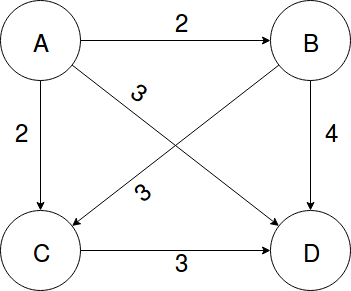
\includegraphics[width=0.35\textwidth]{copeland}
\caption{Majority graph}
\label{fig:copeland}
\end{figure}

La seguente tabella riassume gli esiti di tutti gli scontri tra le coppie
A,B,C,D.

\begin{table}[H]
\begin{tabular}{|c|c|c|c|}
\hline
\textbf{Candidato} & \textbf{Vittorie} & \textbf{Sconfitte} & \textbf{Totale} \\
\hline
A & 1 & 0 & 1 \\ \hline
B & 2 & 0 & 2 \\ \hline
C & 1 & 1 & 0 \\ \hline
D & 0 & 3 & -3 \\ \hline
\end{tabular}
\end{table}

Alcune proprietà desiderabili di questi sistemi sono:

\begin{itemize}
 \item \textbf{Unanimità}: se la prima scelta di tutti gli elettori è
un solo candidato uguale per tutti, allora deve vincere.
 \item \textbf{Non dittatoriali}: non deve esistere un elettore (chiamato
``dittatore'') tale per cui il candidato che è la sua prima scelta vince 
sempre, indipendentemente dai voti degli altri.
 \item \textbf{Non manipolabili}: gli elettori devono essere liberi di
esprimere le loro preferenze, non devono essere manipolabili.
\end{itemize}

Il \textbf{teorema di Arrow} afferma che non è possibile trovare un sistema di 
voto che garantisca contemporaneamente l'unanimità e che non sia dittatoriale.\\

Il \textbf{teorema di Gibbard-Sattherwaite} afferma che non è possibile trovare
un sistema di voto che non sia dittatoriale e anche non manipolabile.\\

Questi teoremi valgono sia nel caso in cui l'insieme delle preferenze sia
totalmente ordinabile sia nel caso in cui sia parzialmente ordinabile.

In molti scenari dell'AI \textbf{multiagente} si hanno situazioni in cui
può succedere che due o più oggetti non siano comparabili (in questo caso
l'insieme delle preferenze è \textbf{parzialmente ordinabile}), che ci sia
incertezza, complessità computazionale e un insieme di oggetti/scelte molto
grande rispetto al numero di agenti.

Ci sono 2 formalismi per far fronte a questa serie di problemi; il primo
è il formalismo dei \textit{soft constraints} che modella preferenze di
tipo quantitativo (numeri) e incondizionate (senza condizioni aggiuntive... ad
esempio, voto X se Y), il secondo è il formalismo delle \textit{CP-net}, che
modella preferenze di tipo qualitativo (preferisco A a B) e condizionate.

In figura \ref{fig:cpnet} è rappresentata una CP-net che modella le preferenze
di una persona per un pasto.

\begin{figure}[H]
\centering
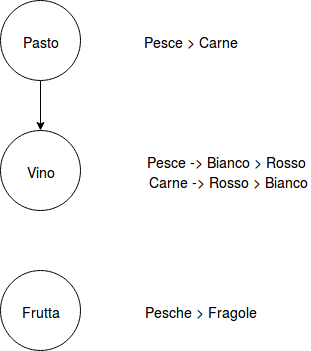
\includegraphics[width=0.35\textwidth]{cpnet}
\caption{Un esempio di CP-net per modellare le preferenze di un
pasto}
\label{fig:cpnet}
\end{figure}

Trovare una soluzione ottima in una CP-net aciclica è semplice\dots

\begin{itemize}
 \item Prima si considerano le variabili indipendenti e si assegna
a loro il valore di preferenza massima.
 \item Poi si considerano le variabili dipendenti e si assegna loro
i valori preferiti in modo consistente ai loro genitori.
\end{itemize}

Nell'esempio si comincia dal pasto e dalla frutta, per finire con
il vino. La soluzione ottima è: \{pasto = Pesce, vino = Bianco,
frutta= Pesche\}\\

Questi 2 formalismi hanno un diverso potere espressivo e richiedono
diverse capacità computazionali.

\begin{table}[H]
\begin{tabular}{|p{3.5cm}|c|c|c|}
\hline
\textbf{Caratteristiche} & \textbf{Soft constraints} & \textbf{CP-Nets} &
\textbf{Acyclic CP-nets} \\ \hline
\textbf{Ordinamento delle preferenze} & totalmente ordinabili & parzialmente
ordinabili & parzialmente ordinabili \\ \hline
\textbf{Trovare una scelta ottima} & difficile & difficile & facile \\ \hline
\textbf{Comparare due scelte} & facile & difficile & difficile \\ \hline
\textbf{Controllare se una scelta è ottima} & difficile & facile & facile \\
\hline
\end{tabular}
\end{table}
